%%%%%%%%%%%%%%%%%%%%%%%%%%%%%%%%%%
% EEE Report Template
% University of Southampton
%
% authors: George Brown (gb4g15)
%          Rhys Thomas  (rt8g15)
%
% edited : 2016/02/05
%%%%%%%%%%%%%%%%%%%%%%%%%%%%%%%%%%

\documentclass[10pt]{article}

%%%%%%%%%%%%%%%%%%%%%%%%%%%%%%%%%%
% PACKAGES
%%%%%%%%%%%%%%%%%%%%%%%%%%%%%%%%%%
\usepackage{multicol} % multiple columns
\usepackage{fancyhdr} % page number in bottom right
\usepackage{graphicx} % images
\usepackage{float} % float image in columns, gives [H]
\usepackage{amsmath, amssymb} % maths symbols / environments
\usepackage{breqn}
\usepackage{times} % times font instead of computer modern
\usepackage{IEEEtrantools} % et al referencing
\usepackage{booktabs} % nice replacements for \hline in tables
\usepackage{calc} % calculating textwidth-2cm etc.
\usepackage[none]{hyphenat} % no hyphenation
\usepackage{geometry} % Page Margins
\usepackage{hyperref} % PDF metadata setup.
\usepackage{mathptmx} % Use times font face for maths
\usepackage{caption} % Tighter caption control.
\usepackage{subcaption}
\usepackage{appendix}
\usepackage{listings}

%https://tex.stackexchange.com/questions/116534/lstlisting-line-wrapping
\usepackage{lmodern}  % for bold teletype font
\usepackage{amsmath}  % for \hookrightarrow
\usepackage{xcolor}   % for \textcolor
\lstset{
  basicstyle=\ttfamily,
  columns=fullflexible,
  frame=single,
  breaklines=true,
  postbreak=\mbox{\textcolor{red}{$\hookrightarrow$}\space},
}

\usepackage{lipsum} % Temporary to generate body text

%%%%%%%%%%%%%%%%%%%%%%%%%%%%%%%%%%
% TITLE AND AUTHOR
%%%%%%%%%%%%%%%%%%%%%%%%%%%%%%%%%%
% This info is reused in places, so input it here and it will be updated globally.
\newcommand{\docTitle}{Whiteboard Chat Applictaion with Half-Duplex Communication}
\newcommand{\docAuthor}{Joesph Butterworth}

% Put the metadata in the PDF output.
\hypersetup{
    unicode=true,
    pdftitle={\docTitle{}},
    pdfauthor={\docAuthor{}}
}

%%%%%%%%%%%%%%%%%%%%%%%%%%%%%%%%%%
% FORMATTING REQUIREMENTS
%%%%%%%%%%%%%%%%%%%%%%%%%%%%%%%%%%
\geometry{top=2.5cm, bottom=2.5cm, left=2cm, right=2cm}
\linespread{1.05} % 1.05x line spacing.
\setlength{\columnsep}{0.7cm} % 0.7cm column spacing.
\setlength{\multicolsep}{0cm}
\setlength{\parskip}{6pt} % 6pt skip between paragraphs
\setlength{\parindent}{0pt}
\newcommand{\figsquish}{\vspace{-5mm}} % Hack to fix poor figure spacing due to [H]

% Captions
% Table captions go above, 6pt space, small (9pt) roman font, roman numeral counting.
%\captionsetup[table]{position=above, skip=6pt, font={small, rm}}
\renewcommand\thetable{\Roman{table}}
% Figure captions go below, 5pt space, small (9pt) roman font.
\captionsetup[figure]{position=below, skip=5pt, font={small, rm}}

% Captions
% Table captions go above, 6pt space, small (9pt) roman font, roman numeral counting.
\captionsetup[table]{position=above, skip=6pt, font={small, rm}}
\renewcommand\thetable{\Roman{table}}
% Figure captions go below, 5pt space, small (9pt) roman font.
\captionsetup[figure]{position=below, skip=5pt, font={small, rm}}

%%%%%%%%%%%%%%%%%%%%%%%%%%%%%%%%%%
% SECTION REQUIREMENTS
%%%%%%%%%%%%%%%%%%%%%%%%%%%%%%%%%%
\usepackage{titlesec}
\titlelabel{\thetitle.\hspace{0.5cm}} % Dot between number and title on sections.
% Format is 10pt, so \large = 12pt, \normalsize=10pt
\titleformat*{\section}{\large\bfseries}
\titlespacing*{\section}{0cm}{4pt}{4pt} % 6pt from \parindent
\titleformat*{\subsection}{\normalsize\bfseries}
\titlespacing*{\subsection}{0cm}{0pt}{0pt} % 6pt from \parindent

% Set up footer.
\pagestyle{fancy}
\fancyhf{}
\renewcommand{\headrulewidth}{0pt}
\rfoot{\thepage} % page number, bottom right of page

%%%%%%%%%%%%%%%%%%%%%%%%%%%%%%%%%%
% DOCUMENT BEGIN
%%%%%%%%%%%%%%%%%%%%%%%%%%%%%%%%%%

\begin{document}

% Pull in the IEEE referencing setup stuff.
\bstctlcite{IEEEexample:BSTcontrol}

%%%%%%%%%%%%%%%%%%%%%%%%%%%%%%%%%%
% HEADER
%%%%%%%%%%%%%%%%%%%%%%%%%%%%%%%%%%
{
    \centering
    % Use size 28 font. 1.05x gives 29.4pt line spacing.
    \fontsize{28pt}{29.4pt} \selectfont
    \docTitle\\
    \vspace{25pt}
    % Name block.
    \fontsize{11pt}{11.55pt}\selectfont
    \docAuthor\\
    \fontsize{10pt}{10.5pt}\selectfont
    \textit{jdb1g20@soton.ac.uk} \\ % add your email address
    \textit{MEng Electrical and Electronic Engineering} \\ 
    \textit{Personal Tutor: Tracy Melvin} \\ % add your personal tutor
}
\vspace{25pt}

%%%%%%%%%%%%%%%%%%%%%%%%%%%%%%%%%%
% ABSTRACT
%%%%%%%%%%%%%%%%%%%%%%%%%%%%%%%%%%
{
\setlength{\tabcolsep}{0cm} % No additional column spacing since we've set it strictly.
\centering
\begin{tabular}{p{2cm}p{\textwidth-2cm}}
    Abstract: &
    
\end{tabular}  
}
\vspace{25pt}

%%%%%%%%%%%%%%%%%%%%%%%%%%%%%%%%%%
% BODY
%%%%%%%%%%%%%%%%%%%%%%%%%%%%%%%%%%
\begin{multicols*}{2}

\section{Introduction}

\section{Theory}
\subsection{QPainter}
How will the send-window allow users to draw diagrams? How will it display
diagrams as they are being drawn, and how will it retain these diagrams so
that they don’t disappear when the window is repainted?

QPainter is a part of the qt library family that allows you to draw pixel graphics. For this application, QPainter will be used to modify a QImage.

\subsection{Threads and Mutexes}
text

How will you use threads to send and receive these packets, while the rest of
the application keeps running? How will you use mutexes to make any relevant
collections “thread-safe”?

\subsection{Serialisation}
How will you serialize these commands into packets to be sent from the send
window?

How will you convert binary packets into a stream of 1’s and 0’s? How will you
transmit this stream in a reliable way? For example, you may need to signal
when a bit is ready to be read, and when the receive window has finished
reading the current bit.

\subsection{Simplex, Half-Duplex, and Duplex Communication}
How will you represent the drawing commands so that they can be sent to the
other user whilst they are being drawn?

How will you receive and buffer packets at the other end? How will you
deserialize them? How will you draw them on the receive window? How will
you retain the currently received diagram so that when the window is
repainted the diagram isn’t lost?

\subsection{Class Architecture of the Whiteboard Applicatoin}

\section{Implementation}
\subsection{The GUI - Send and Receive Window}
On initiasation, the program creates new instances of the sendWindow and receiveWindow classes. The new windows are then given defined parameters, they are named and resized to a proportion of the screen they are being displayed on.
$\\$ \figsquish
\begin{lstlisting}[language=C++]
QScreen *screen = 
	QGuiApplication::primaryScreen();
QRect  screenGeometry = screen->geometry();
int height = screenGeometry.height();
int width = screenGeometry.width();

// Creating send window
QPixmap sendpix(QDir::currentPath() 
	+ "/Icons/send_icon.png");

sendWindow sendW(nullptr);
sendW.setWindowIcon(sendpix);
sendW.setWindowTitle("Send Window");
sendW.resize(width/3, height/2);
sendW.move(width/9, height/4);
sendW.show();
\end{lstlisting}
\figsquish $\\$
The sendWindow and receiveWindow classes inhereted from QMainWindow. To enable either the user or the draw commands the central widgets were set to be their respective canvas classes, sendCanvas and receiveCanvas.
$\\$ \figsquish
\begin{lstlisting}[language=C++]
sendCanvas::sendCanvas(QWidget *parent)
	: QWidget(parent)
\end{lstlisting}
\figsquish $\\$
The central canvases would draw by taking the position of an input, for the send window a mouse click and for the receive window the position data passed to it by the send window, and drawing a rectangle between them. For the send window the mousePressEvent(), mouseMoveEvent() and mouseReleaseEvent() were all overwritten. The program is able to draw curves and circles owing to the mouseMoveEvent() function being overwritten, this receives a lot of information from the mouse as it is constantly polling, hence all the rectangles are really small and to create a smooth line.
$\\$ \figsquish
\begin{lstlisting}[language=C++]
QPainter painter(&drawImage);

// Create pen and draw line
QPen newPen(areaBrushStyle, areaPenWidth, 
	areaPenStyle, areaCapStyle, 
	Qt::RoundJoin);
newPen.setColor(areaColour);    
painter.setPen(newPen);
painter.drawLine(prevPoint, endPoint);

// Maintain radius whilst drawing
int radius = (areaPenWidth / 2) + 2;
update(QRect(prevPoint, endPoint)
	.normalized().adjusted(-radius,
	 -radius, +radius, +radius));

// Update point
prevPoint = endPoint;
\end{lstlisting}
\figsquish $\\$
When using the drawLine() function the program uses QPainter to draw a line from the last known position to the new position. It maintains the previous drawings by loading an image of the previous inputs, the private variable drawImage, as the canvas and overlaying the new rectangle on top of that. 

In addition to the central UI of the canvas, the send window also has a menubar and toolbar that allows users to easily interact with the program as in Figure \ref{fig:menus}, in an easy to use fashion. The user inputs used the QMenubar and QToolbar functionality, to easily add buttons to the menubar and toolbar.
$\\$ \figsquish
\begin{lstlisting}[language=C++]
// Toolbar
auto *colour = new QAction("&Colour", this);
auto *width = new QAction("&Pen Width", this);

QToolBar *toolbar = 
	addToolBar("main toolbar");
toolbar->addAction(colour);
toolbar->addSeparator();
toolbar->addAction(width);

connect(colour, &QAction::triggered, this, 
	&sendWindow::colour);
connect(width, &QAction::triggered, this, 
	&sendWindow::penWidth);
\end{lstlisting}
\figsquish $\\$
These buttons were connected to member functions, that used the QFileDialog, QInputDialog and QColorDialog, this allowed for effective handling of opening files, saving the screen as an image, getting the pen width and the pen colour respectively, shown in Figures \ref{fig:fileDialogs} \& \ref{fig:drawDialogs}. Using the Qt library family allowed the program to use dialog boxes in a way that would be familiar to any user. 
$\\$ \figsquish
\begin{lstlisting}[language=C++]
// Get image file formats
const QList<QByteArray> imageFormats = 
	QImageWriter::supportedImageFormats();

// Create file filter from QList
QString fileFilter = "";
for(const QByteArray &format : imageFormats)
{
     fileFilter.append(tr("%1 Files (*.%2)")
	.arg(QString::fromLatin1(format)
	.toUpper(), 
	QString::fromLatin1(format)));
    fileFilter.append(";;");
}
//qDebug() << fileFilter;

// Set filename from dialog box
QString fileName = 
	QFileDialog::getSaveFileName(this, 
	tr("Save File"), QDir::currentPath() 
	+ "/untitled", fileFilter);

// Set fileformat from dialog box
char *format = fileName.split(".").last()
	.toUtf8().data();

// Pass to draw area function
if (!fileName.isEmpty())
        canvas->saveArea(fileName, format);
\end{lstlisting}
\figsquish $\\$

\subsection{The Serialise and Deserialise Drawing Commands}
To pass the positional data between classes a struct using uint16\_ts was used. This was very similar to passing a QPoint between objects. However, this limited the size of the information, so that it is larger than the screen is likely to be but to smaller than passing entire ints across.
$\\$ \figsquish
\begin{lstlisting}[language=C++]
typedef struct drawInfoPosition
{
    // Opcodes
    // Bit 1 for odd-on parity
    uint8_t opcode;

    // Vertical and Horizontal Positions
    uint16_t xPosition;
    uint16_t yPosition;

} drawInfoPosition;
\end{lstlisting}
\figsquish $\\$
The drawInfoPosition struct could easily be serialised by loopiing over every element and pushing it to a boolean array. This is now the sequential series that can be pushed across a pin or onto a threadsafe queue.
$\\$ \figsquish
\begin{lstlisting}[language=C++]
uint16_t temp[3] = {serialData.opcode, 
	serialData.xPosition, 
	serialData.yPosition};
bool serialsedArray[48];

// Loop over each element of the 
//temporary array
for(int i = 0; i < 3; i++)
{
    for(int j = 15; j>= 0; j--)
    {
        // Convert to binary
        if (temp[i] >= pow(2, j))
       {

            temp[i] -= pow(2, j);

            // Increase Local Count
            serialsedArray[i*j+j] = true;
        }
    }
}
\end{lstlisting}
\figsquish $\\$
Likewise the boolean array can be deserialised when it is received back into a drawInfoPosition struct, from which a QPoint can be constructed.
$\\$ \figsquish
\begin{lstlisting}[language=C++]
drawInfoPosition serialData;
uint16_t temp[3] = {serialData.opcode, 
	serialData.xPosition, 
	serialData.yPosition};

// Loop over each element of the 
//temporary array
for(int i = 0; i < 3; i++)
{
    for(int j = 15; j>= 0; j--)
   {
       // Convert to decimal
       if (serialsedArray[i*i+j])
       {
           temp[i] += pow(2,j);
        }
    }
}
\end{lstlisting}
\figsquish $\\$
\subsection{The Send and Receive Threads}
To pass the serialised information across without using a large thread overhead worker threads have to be used. As the send and receive canvases are the classes that use the positional information it would be effeceint to send the information directly between them. Hence, the worker threads to the send and receive window should be instantiated in the send and receive canvases.
$\\$ \figsquish
\begin{lstlisting}[language=C++]
sendThread *worker = new sendThread();
worker->moveToThread(&sender);
connect(&sender, &QThread::finished, worker, 
	&QObject::deleteLater);
connect(this, 
	SIGNAL(drawSignal(drawInfoPosition)), 
	worker, SLOT(pushSerialStruct(
	drawInfoPosition)));
sender.start();
\end{lstlisting}
\figsquish $\\$
The send and receive threads cannot directly communicate with each other using signals and slots as they cannot be referenced to each other. As such they require an entity in common that they may both interact with. To allow this communication a thread safe queue class template was to be implemented to allow easy communication between the threads.

However, the threadsafe queue that was implemented failed to initialise correctly and either created a compile error $undefiened\ reference\ to\ vtable$ or worse would compile then give a SIGSEGV error when opening. A large portion of the time spent on this project was spent trying to resolve this issue. The errors in the queue class template were never resolved. Therefore, the send and receive thread were never able to communicate.

\subsection{Communication Protocol using Booleans}
Despite the inability for the threads to communicate there was still progress in creating a communication protocol.



\section{Final Application}

\begin{figure}[H]
	\centering
	\begin{subfigure}[t]{0.48\columnwidth}

		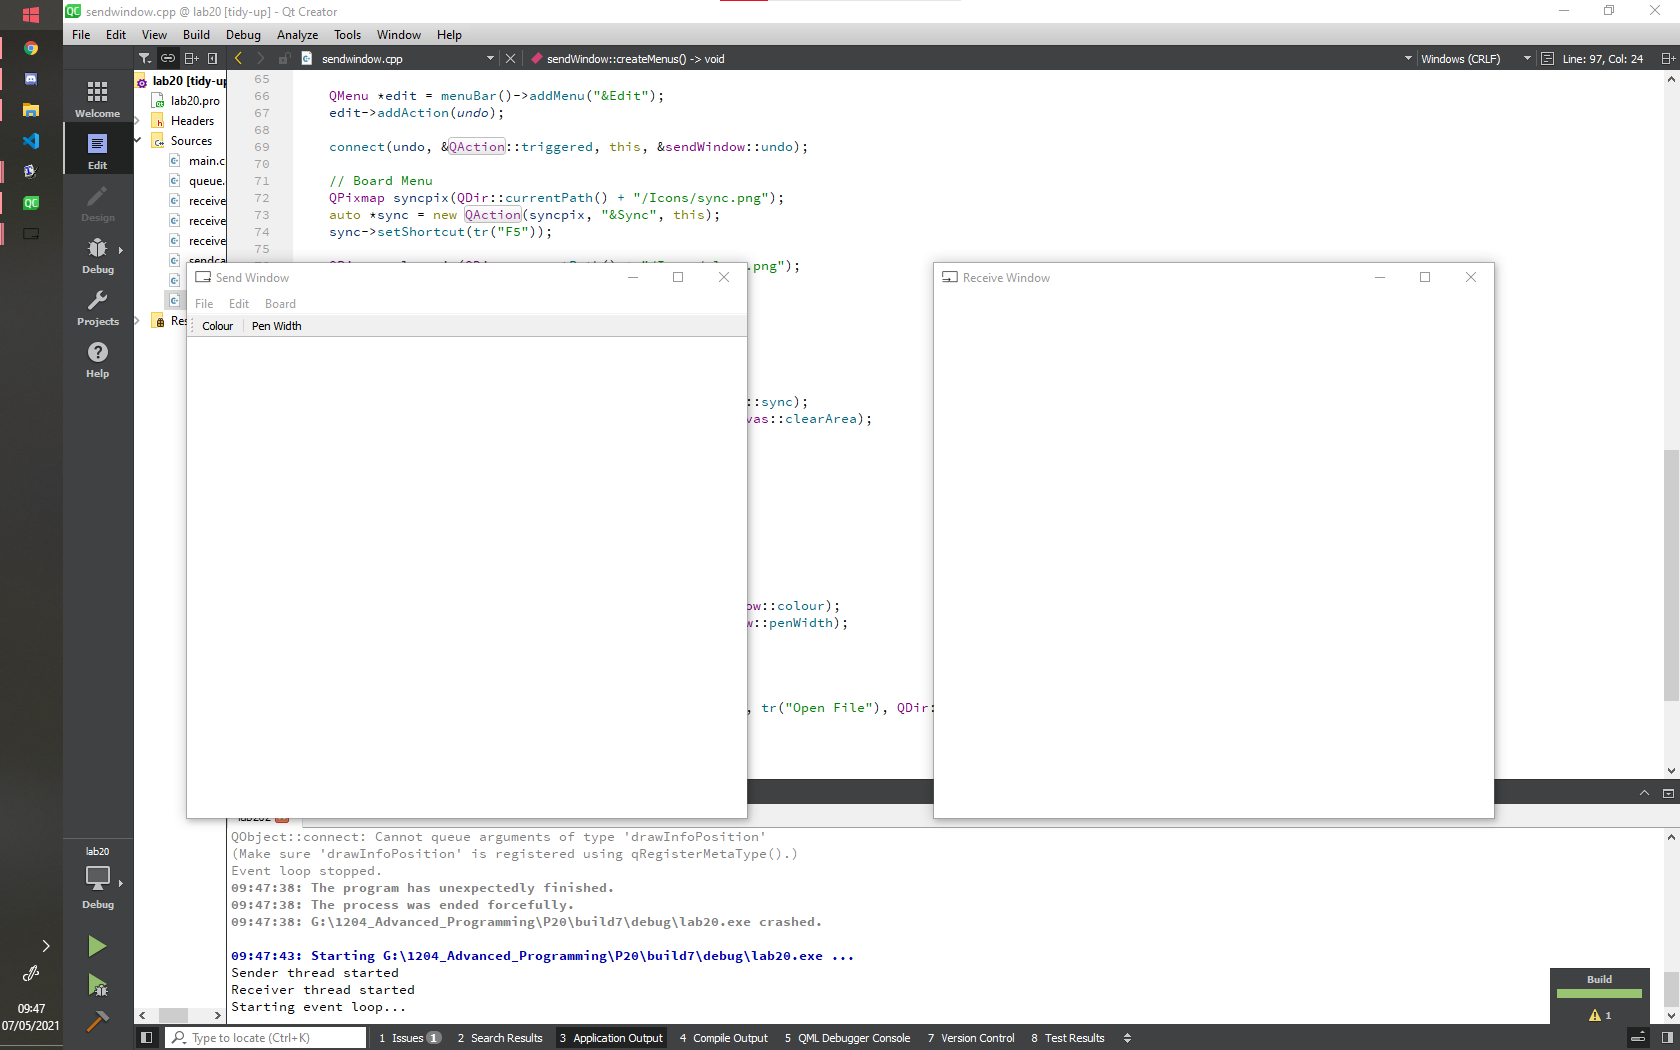
\includegraphics[width=\columnwidth]{./application.png}
		\caption{Send and receive windows when application is opened}
		\label{fig:app}
	\end{subfigure}
	\hfill
	\begin{subfigure}[t]{0.48\columnwidth}

		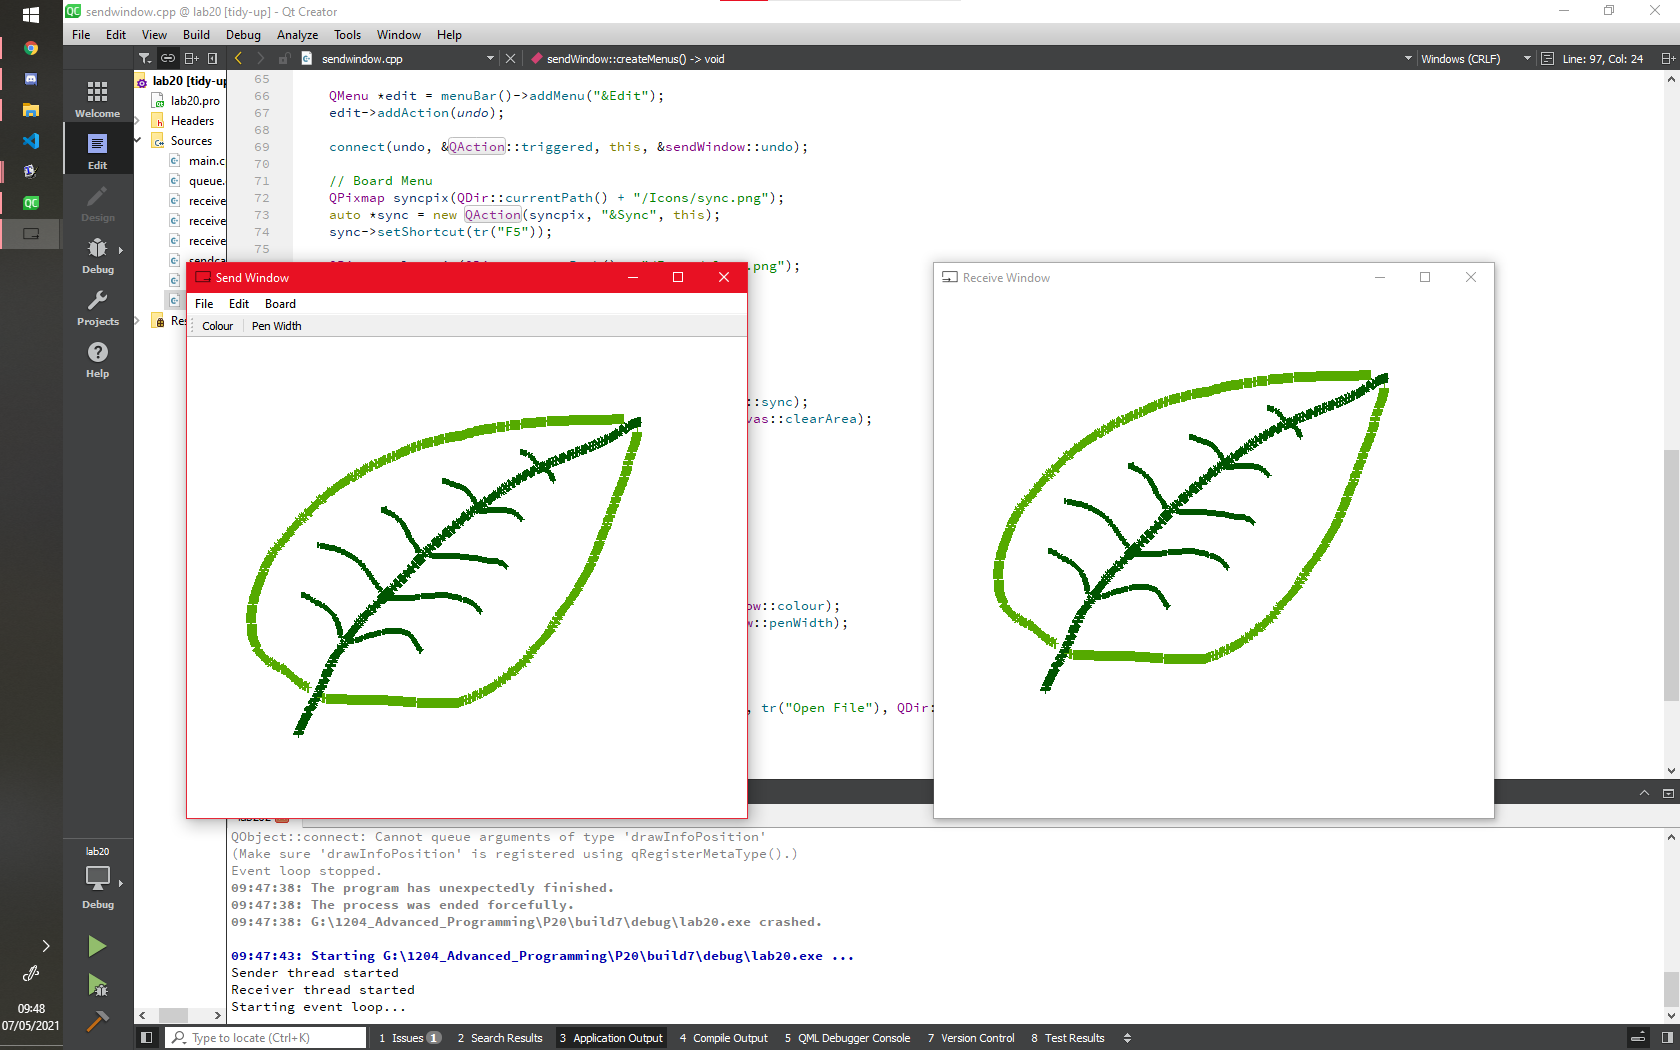
\includegraphics[width=\columnwidth]{./application drawing.png}
		\caption{Send and receive windows after drawing}
		\label{fig:app-drawing}
	\end{subfigure}
	\caption{Send and receive windows open on screen and allow drawing between them}
	\label{fig:application}
\end{figure}
\figsquish

\begin{figure}[H]
	\centering
	\begin{subfigure}[t]{0.32\columnwidth}

		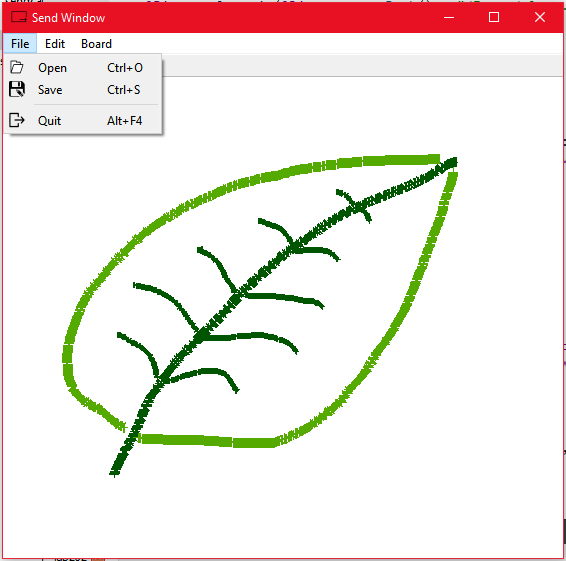
\includegraphics[width=\columnwidth]{./file.png}
		\caption{File Menu with  opening saving and closing}
		\label{fig:file}
	\end{subfigure}
	\hfill
	\begin{subfigure}[t]{0.32\columnwidth}

		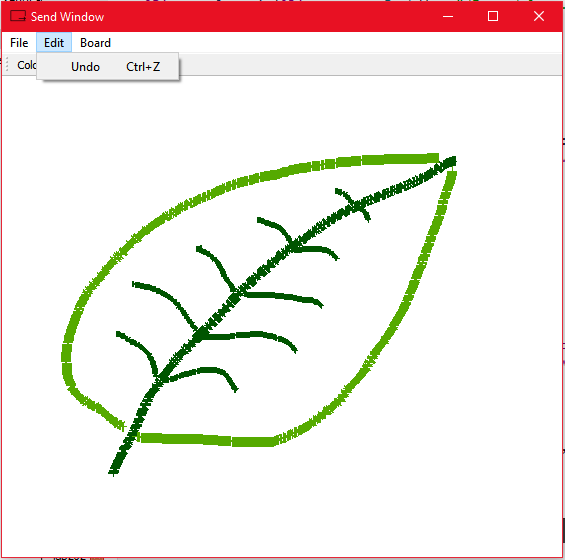
\includegraphics[width=\columnwidth]{./edit.png}
		\caption{Edit Menu with the undo functionality, redo was to be added later}
		\label{fig:edit}
	\end{subfigure}
	\hfill
	\begin{subfigure}[t]{0.32\columnwidth}

		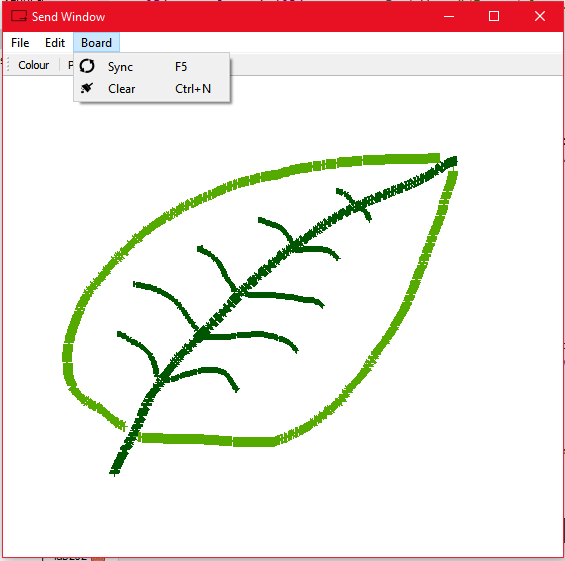
\includegraphics[width=\columnwidth]{./board.png}
		\caption{Board menu allows the screen to be cleared or windows to be synced}
		\label{fig:board}
	\end{subfigure}
	\caption{Menus allow the user to control the program}
	\label{fig:menus}
\end{figure}
\figsquish

\begin{figure}[H]
	\centering
	\begin{subfigure}[t]{0.48\columnwidth}

		
\includegraphics[width=\columnwidth]{./open.png}
		\caption{Open file dialog}
		\label{fig:open}
	\end{subfigure}
	\hfill
	\begin{subfigure}[t]{0.48\columnwidth}

		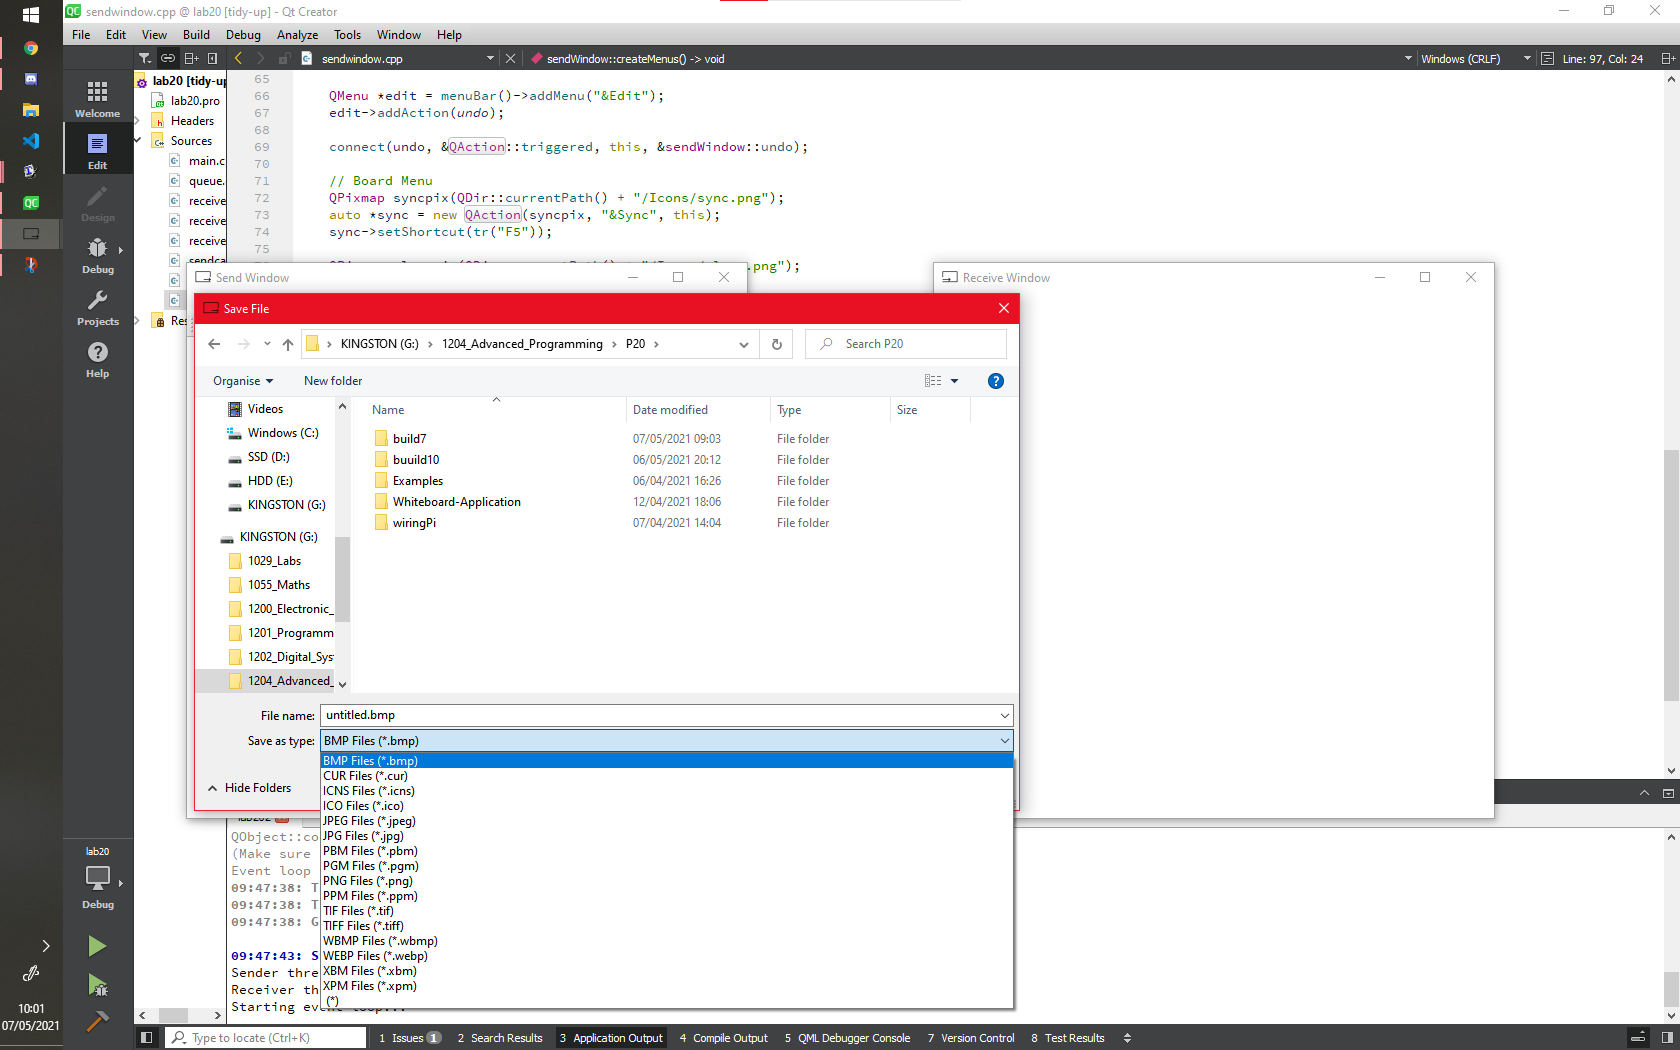
\includegraphics[width=\columnwidth]{./save.png}
		\caption{Save file dialog}
		\label{fig:save}
	\end{subfigure}
	\caption{File handling dialogs using QFileDialog}
	\label{fig:fileDialogs}
\end{figure}
\figsquish

\begin{figure}[H]
	\centering
	\begin{subfigure}[t]{0.48\columnwidth}

		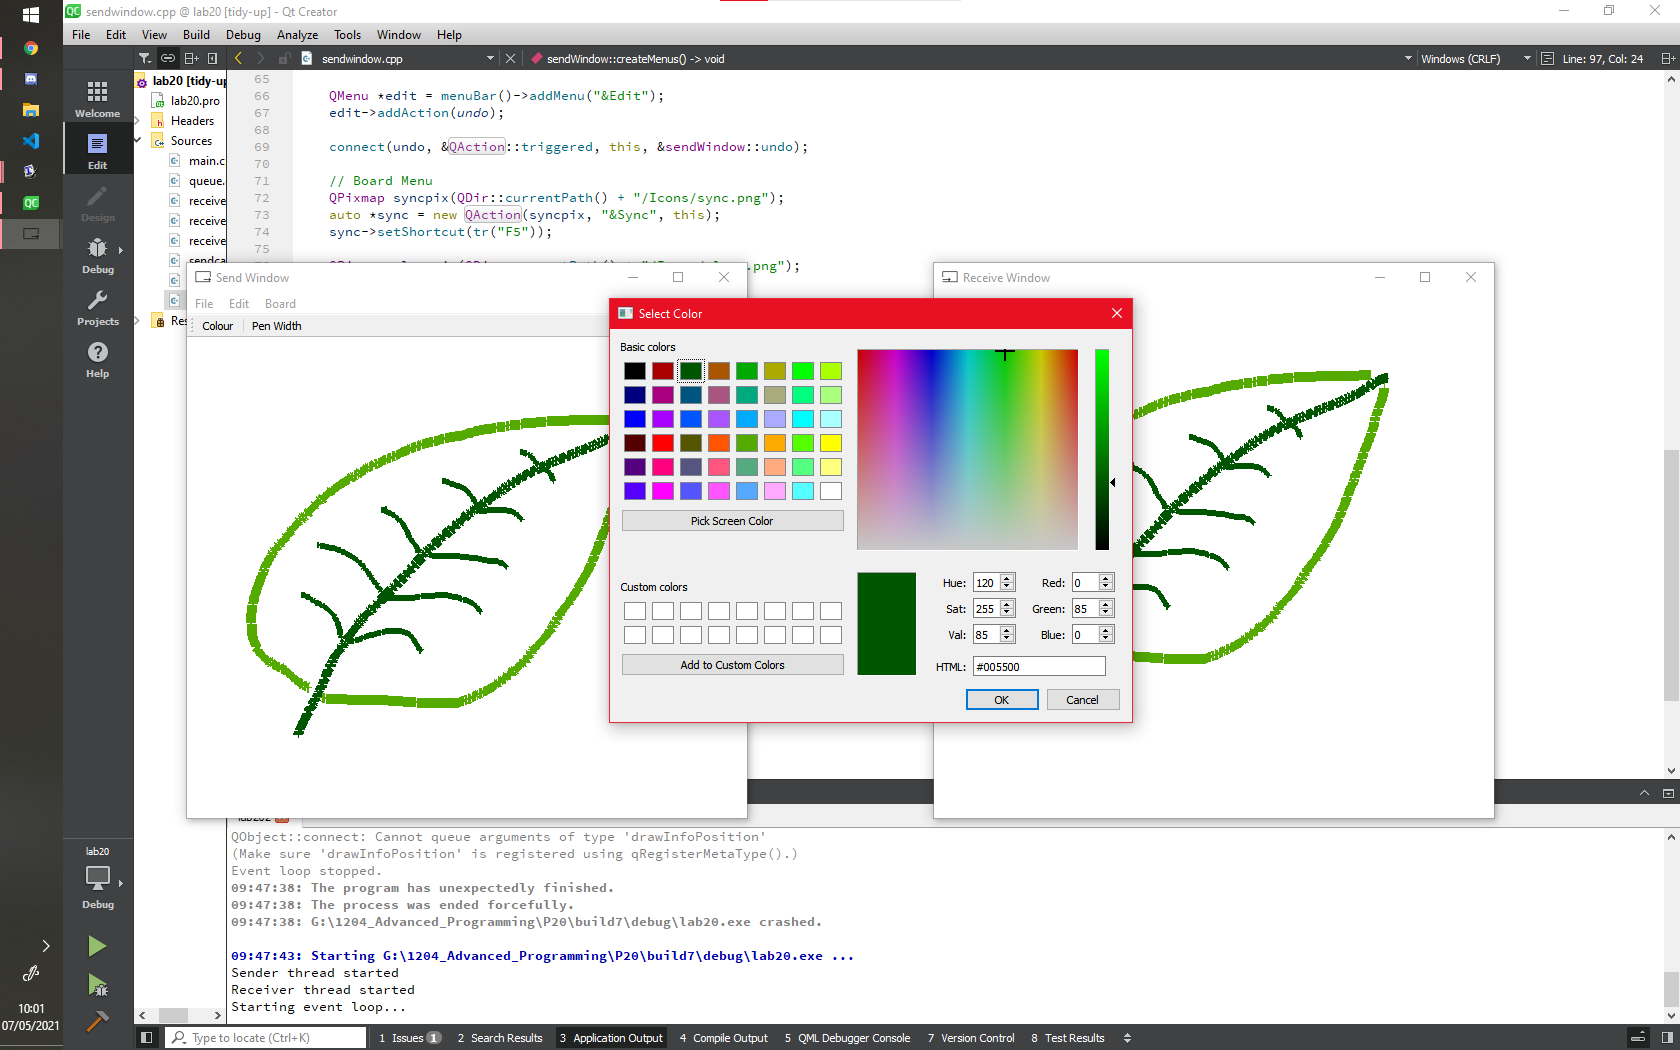
\includegraphics[width=\columnwidth]{./colour.png}
		\caption{Colour selection dialog box}
		\label{fig:colour}
	\end{subfigure}
	\hfill
	\begin{subfigure}[t]{0.48\columnwidth}

		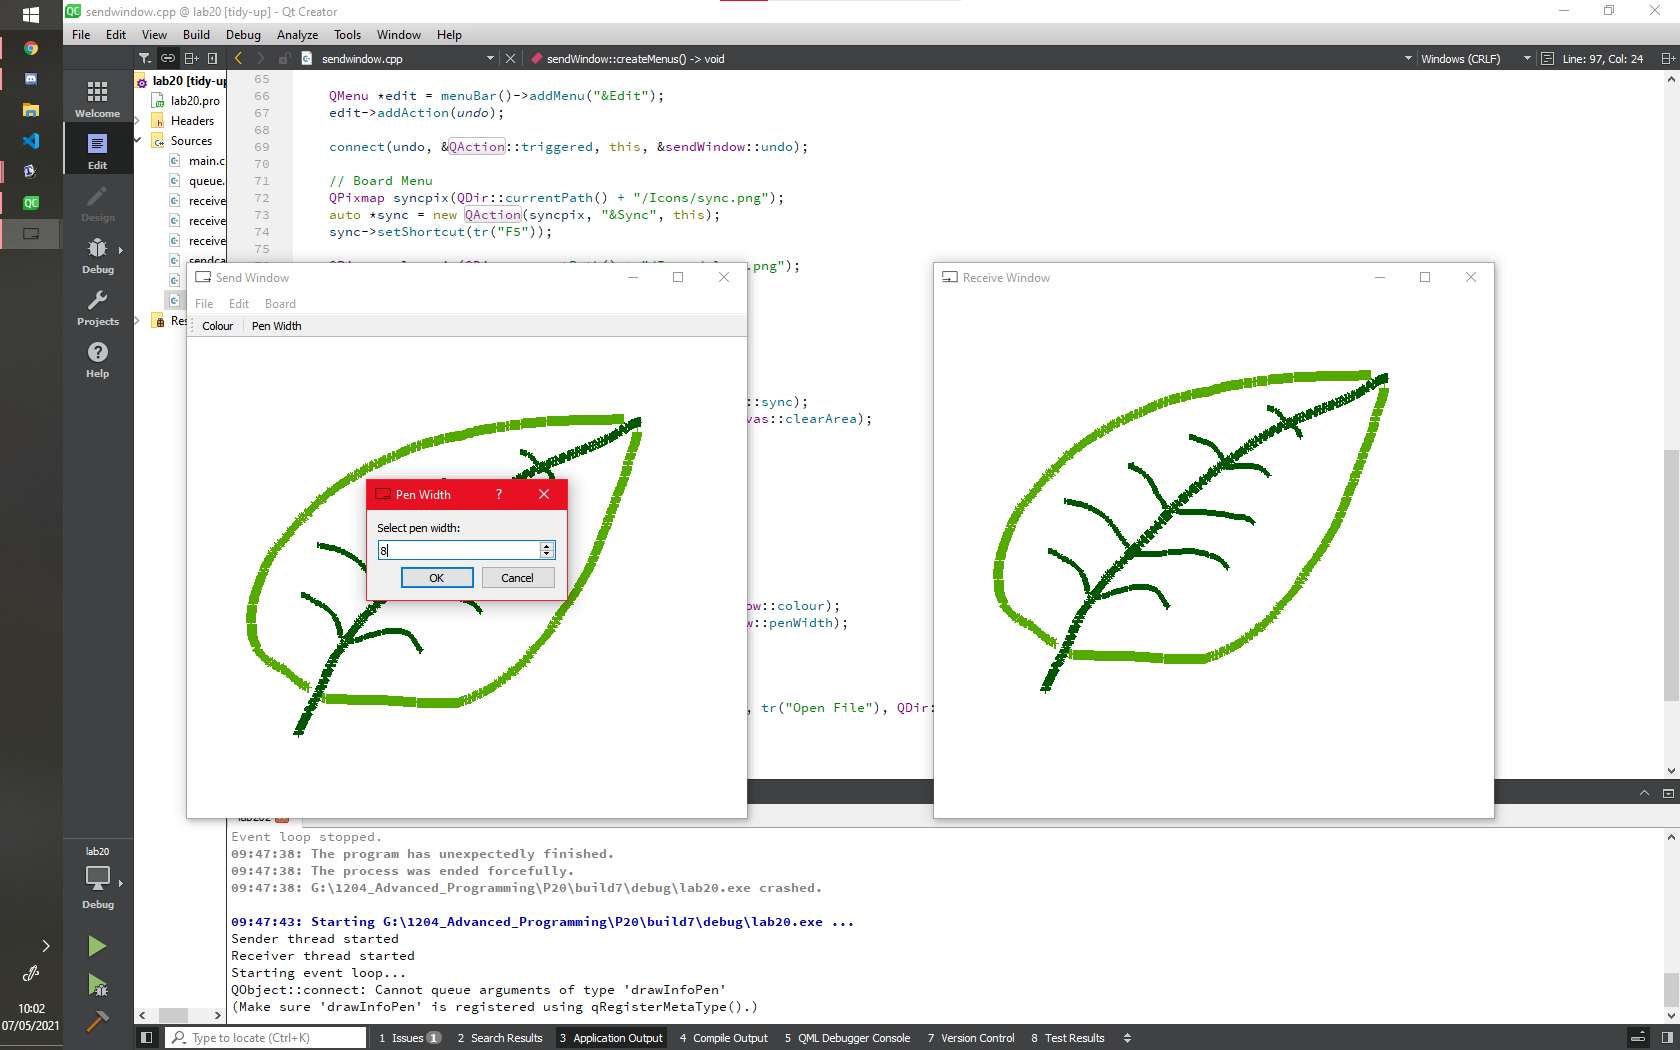
\includegraphics[width=\columnwidth]{./width.png}
		\caption{Pen width control dialog box}
		\label{fig:width}
	\end{subfigure}
	\caption{Dialog boxes to control the QPen characteristics}
	\label{fig:drawDialogs}
\end{figure}
\figsquish


\section{Discussion}

\section{Conclusion}


%%%%%%%%%%%%%%%%%%%%%%%%%%%%%%%%%%
% BIBLIOGRAPHY
%%%%%%%%%%%%%%%%%%%%%%%%%%%%%%%%%%
\nocite{*} % show all references even without citation
% to cite use "bla bla"~\cite{ref_label} -> "bla bla" [1]
\bibliographystyle{IEEEtran}
% IEEEabrv abbreviates journal titles in accordance to IEEE standards 
\bibliography{IEEEabrv,mybib}

\end{multicols*}
\end{document}
